\documentclass{standalone}
\usepackage{picture,color}
\usepackage{graphicx}
\graphicspath{{./FIG_BNST_subfigs/}}
\setlength{\unitlength}{1in}
% \definecolor{red}{rgb}{   0.4039, 0, 0.0510}
% \definecolor{green}{rgb}{  0, 0.2667, 0.1059}
\usepackage{helvet}
\renewcommand{\familydefault}{\sfdefault}

\begin{document}
\begin{picture}(6.8,7.9)(0.05,-5.91)

\put(1.75, -0.08){\includegraphics[height=1.9in]{FIG_BNST_subfigs/cnmfe_colorbar.png}}
\put(0.4, 0.01){\includegraphics[height=1.75in]{FIG_BNST_subfigs/cnmfe_match_spatial.pdf}}
\put(0.1, 1.75){\large\textbf{A}}
\put(0.8, 1.8){\normalsize CNMF-E}

\put(3.65, -0.08){\includegraphics[height=1.9in]{FIG_BNST_subfigs/ica_colorbar.png}}
\put(2.3, 0.01){\includegraphics[height=1.75in]{FIG_BNST_subfigs/ica_match_spatial.pdf}}
\put(2.7, 1.8){\normalsize PCA/ICA}

\put(0.1, -2.1){\includegraphics[height=1.8in]{FIG_BNST_subfigs/cnmfe_match_temporal.pdf}}
\put(3., -0.25){\normalsize Temporal traces}
\put(0.1, -3.6){\includegraphics[height=1.8in]{FIG_BNST_subfigs/ica_match_temporal.pdf}}
\put(6.65, -1.4){\rotatebox{90}{{\normalsize CNMF-E}}}
\put(6.65, -2.9){\rotatebox{90}{{\normalsize PCA/ICA}}}
\put(0.1, -0.3){\large\textbf{C}}

% contours  
\put(4.4, -0.15){\includegraphics[height=1.92in]{FIG_BNST_subfigs/match_contours.pdf}}
\put(4.75, 1.8){\normalsize Correlation image}
\put(4.2, 1.75){\large\textbf{B}}

% example neurons 
\put(0.07, -5.9){\includegraphics[height=2.35in]{FIG_BNST_subfigs/shock_neuron_1.pdf}}
\put(0.74, -5.9){\includegraphics[height=2.35in]{FIG_BNST_subfigs/shock_neuron_2.pdf}}
\put(1.15, -5.9){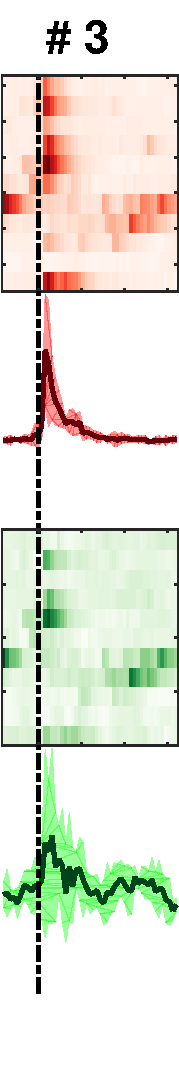
\includegraphics[height=2.35in]{FIG_BNST_subfigs/shock_neuron_3.pdf}}
\put(1.56, -5.9){\includegraphics[height=2.35in]{FIG_BNST_subfigs/shock_neuron_4.pdf}}
\put(1.97, -5.9){\includegraphics[height=2.35in]{FIG_BNST_subfigs/shock_neuron_5.pdf}}
\put(2.38, -5.9){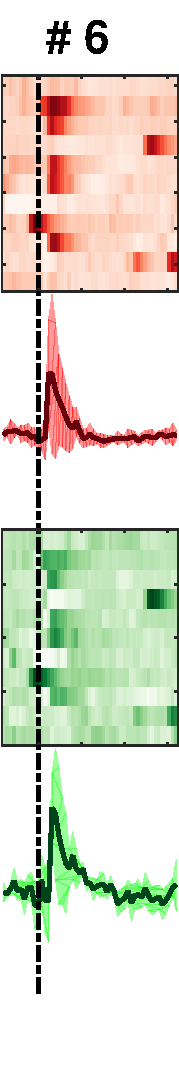
\includegraphics[height=2.35in]{FIG_BNST_subfigs/shock_neuron_6.pdf}}
\put(2.79, -5.9){\includegraphics[height=2.35in]{FIG_BNST_subfigs/shock_neuron_7.pdf}}
\put(3.20, -5.9){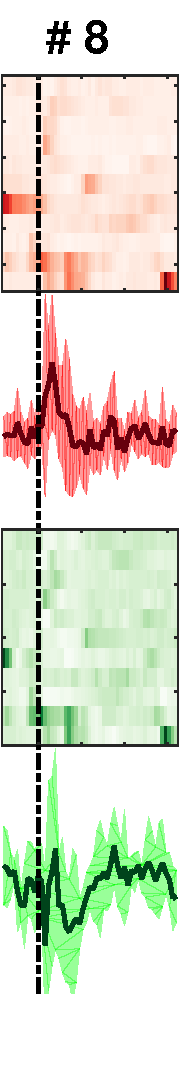
\includegraphics[height=2.35in]{FIG_BNST_subfigs/shock_neuron_8.pdf}}
\put(3.61,  -5.9){\includegraphics[height=2.35in]{FIG_BNST_subfigs/shock_neuron_9.pdf}}
\put(4.02, -5.9){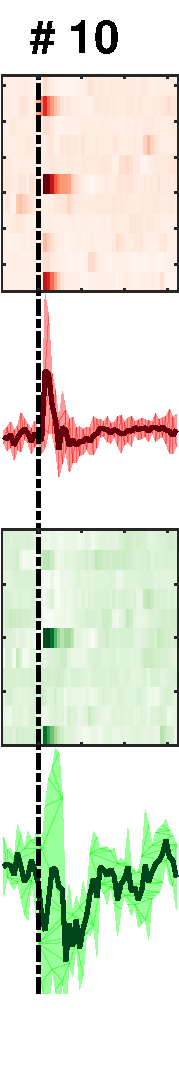
\includegraphics[height=2.35in]{FIG_BNST_subfigs/shock_neuron_10.pdf}}
\put(4.43, -5.9){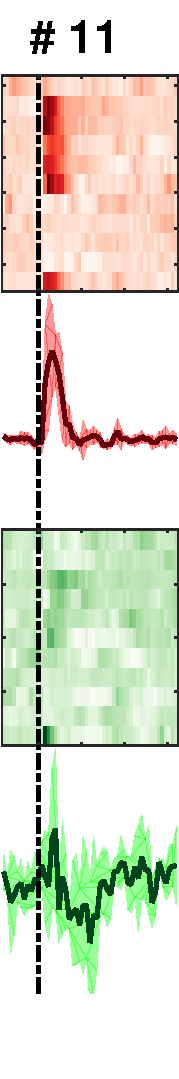
\includegraphics[height=2.35in]{FIG_BNST_subfigs/shock_neuron_11.pdf}}
\put(4.84, -5.9){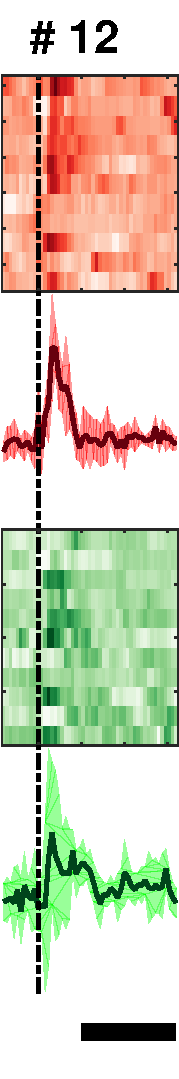
\includegraphics[height=2.35in]{FIG_BNST_subfigs/shock_neuron_12.pdf}}
\put(0.1, -3.6){\large\textbf{D}}
% \put(8.4, -3.5){\rotatebox{90}{\color{red}\textbf{\footnotesize CNMF-E}}}
% \put(8.4, -4.56){\rotatebox{90}{\color{green}\textbf{\footnotesize PCA/ICA}}}

\put(8.4, -3.5){\rotatebox{90}{{\footnotesize CNMF-E}}}
\put(8.4, -4.56){\rotatebox{90}{{\footnotesize PCA/ICA}}}

\put(5.3, -5.65){\includegraphics[height=2.05in]{FIG_BNST_subfigs/shock_peak.pdf}}
\put(5.3, -3.6){\large\textbf{E}}
\put(5.5, -3.65){\normalsize{Peak-to-MAD ratio}}
\end{picture}
\end{document}
